% Options for packages loaded elsewhere
\PassOptionsToPackage{unicode}{hyperref}
\PassOptionsToPackage{hyphens}{url}
%
\documentclass[
]{article}
\title{Ársskýrsla}
\usepackage{etoolbox}
\makeatletter
\providecommand{\subtitle}[1]{% add subtitle to \maketitle
  \apptocmd{\@title}{\par {\large #1 \par}}{}{}
}
\makeatother
\subtitle{\textless br️\textgreater{} náttúrustofu Norðurlands vestra}
\author{}
\date{\vspace{-2.5em}}

\usepackage{amsmath,amssymb}
\usepackage{lmodern}
\usepackage{iftex}
\ifPDFTeX
  \usepackage[T1]{fontenc}
  \usepackage[utf8]{inputenc}
  \usepackage{textcomp} % provide euro and other symbols
\else % if luatex or xetex
  \usepackage{unicode-math}
  \defaultfontfeatures{Scale=MatchLowercase}
  \defaultfontfeatures[\rmfamily]{Ligatures=TeX,Scale=1}
\fi
% Use upquote if available, for straight quotes in verbatim environments
\IfFileExists{upquote.sty}{\usepackage{upquote}}{}
\IfFileExists{microtype.sty}{% use microtype if available
  \usepackage[]{microtype}
  \UseMicrotypeSet[protrusion]{basicmath} % disable protrusion for tt fonts
}{}
\makeatletter
\@ifundefined{KOMAClassName}{% if non-KOMA class
  \IfFileExists{parskip.sty}{%
    \usepackage{parskip}
  }{% else
    \setlength{\parindent}{0pt}
    \setlength{\parskip}{6pt plus 2pt minus 1pt}}
}{% if KOMA class
  \KOMAoptions{parskip=half}}
\makeatother
\usepackage{xcolor}
\IfFileExists{xurl.sty}{\usepackage{xurl}}{} % add URL line breaks if available
\IfFileExists{bookmark.sty}{\usepackage{bookmark}}{\usepackage{hyperref}}
\hypersetup{
  pdftitle={Ársskýrsla},
  hidelinks,
  pdfcreator={LaTeX via pandoc}}
\urlstyle{same} % disable monospaced font for URLs
\usepackage[margin=1in]{geometry}
\usepackage{longtable,booktabs,array}
\usepackage{calc} % for calculating minipage widths
% Correct order of tables after \paragraph or \subparagraph
\usepackage{etoolbox}
\makeatletter
\patchcmd\longtable{\par}{\if@noskipsec\mbox{}\fi\par}{}{}
\makeatother
% Allow footnotes in longtable head/foot
\IfFileExists{footnotehyper.sty}{\usepackage{footnotehyper}}{\usepackage{footnote}}
\makesavenoteenv{longtable}
\usepackage{graphicx}
\makeatletter
\def\maxwidth{\ifdim\Gin@nat@width>\linewidth\linewidth\else\Gin@nat@width\fi}
\def\maxheight{\ifdim\Gin@nat@height>\textheight\textheight\else\Gin@nat@height\fi}
\makeatother
% Scale images if necessary, so that they will not overflow the page
% margins by default, and it is still possible to overwrite the defaults
% using explicit options in \includegraphics[width, height, ...]{}
\setkeys{Gin}{width=\maxwidth,height=\maxheight,keepaspectratio}
% Set default figure placement to htbp
\makeatletter
\def\fps@figure{htbp}
\makeatother
\setlength{\emergencystretch}{3em} % prevent overfull lines
\providecommand{\tightlist}{%
  \setlength{\itemsep}{0pt}\setlength{\parskip}{0pt}}
\setcounter{secnumdepth}{-\maxdimen} % remove section numbering
\ifLuaTeX
  \usepackage{selnolig}  % disable illegal ligatures
\fi

\begin{document}
\maketitle

class: title-slide split-90

\# .font5.font-dance.yellow{[}Ársskýrsla{]} \#\#
.font2.yellow{[}Náttúrustofu Norðurlands vestra{]}
.pull-right{[}.pull-right{[}.pull-right.Large.white{[}
.img-fill{[}
\includegraphics{myndir/nnvlogo.png}{]} 2021{]}{]}{]}

\begin{longtable}[]{@{}
  >{\raggedright\arraybackslash}p{(\columnwidth - 0\tabcolsep) * \real{0.06}}@{}}
\toprule
\begin{minipage}[b]{\linewidth}\raggedright
class: class: split-two with-thick-border border-white duke-softblue
\end{minipage} \\
\midrule
\endhead
class: split-60 with-border name: inngangur .column{[}.content{[} \#
.font-dance{[}Inngangur{]} \\
Starf Náttúrustofu Norðurlands vestra í ár var að venju fjölbreytt og
áhugavert. Farið var víða um landshlutann til náttúruathugana og
rannsókna enda er af nógu að hyggja á landsvæði sem spannar 13.105
km2. \\
Viðfangsefni Náttúrustofunnar snérust að miklu leyti um vöktun náttúru
svæðisins, dýra- og plöntulífs og jarðminja auk þess að svara almennum
fyrirspurnum, hjúkra villtum dýrum í neyð og taka þátt í fræðslu
ungmenna á svæðinu. Fylgst var með fuglum sem og ágengum plöntutegundum
ásamt ágengum dýrum, líkt og minkum og refum. \\
Um vorið voru gerðar athuganir á gæsum yfir landsvæðið þvert og
endilangt, frá Fljótum í Skagafirði til Bitrufjarðar á Ströndum. Eins
var farið norður á Skaga og suður að Ingólfsskála og að Hofsjökli til að
skoða jökulröndina en þaðan er uppganga á jökulinn hvað auðveldust.
Jafnframt var farið um heiðalöndin yfir sumarið og athuganir gerðar á
Arnarvatnsheiði og við Orravatnsrústir á Stórasandi. \\
Náttúrustofan hefur unnið mikið starf við verkefnið „Vöktun
náttúruverndarsvæða`` sem er leitt af Náttúrufræðistofnun Íslands og
unnið í samstarfi við allar náttúrustofur landsins. Gerðar voru úttektir
á náttúruverndarstöðum og ferðamannastöðum til að meta ástand þeirra og
mögulegar ógnir sem að þeim sækja og fylgja gjarnan auknum
ferðamannastraumi, sérstaklega ef innviði vantar og eftirliti er
ábótavant. Náttúruverndarsvæði Norðurlands vestra og aðrir vinsælir
ferðamannastaðir eru mikil verðmæti sem skapa miklar tekjur í
ferðamennsku. Þeir hafa mikið gildi í sjálfu sér og eru
framtíðarverðmæti komandi kynslóða. \\
Á Norðurlandi vestra eru þónokkur náttúruverndarsvæði og allmörg önnur
svæði sem ekki njóta beinnar náttúruverndar en teljast afar mikilvæg
fyrir náttúru Íslands. Má hér til dæmis nefna hin víðáttumiklu vatna- og
heiðasvæði Guðlaugstungur og Arnarvatnsheiði og einnig Skagaheiðina,
Eylendið í Skagafirði eða Flóðið og Eylendið í Vatnsdal, fuglabjörgin í
Drangey og Málmey. Strandlónin Höfðavatn og Sigríðarstaðavatn bera
einnig mikið og fjölbreytt fuglalíf. Það hefur fallið að nokkru leyti í
hlut Náttúrustofunnar að fylgjast með náttúrufari á þessum stöðum og
sinna rannsóknum og eftirliti. \\
{]}{]} \\
.column{[}.content.nopadding{[} \\
.img-fill{[}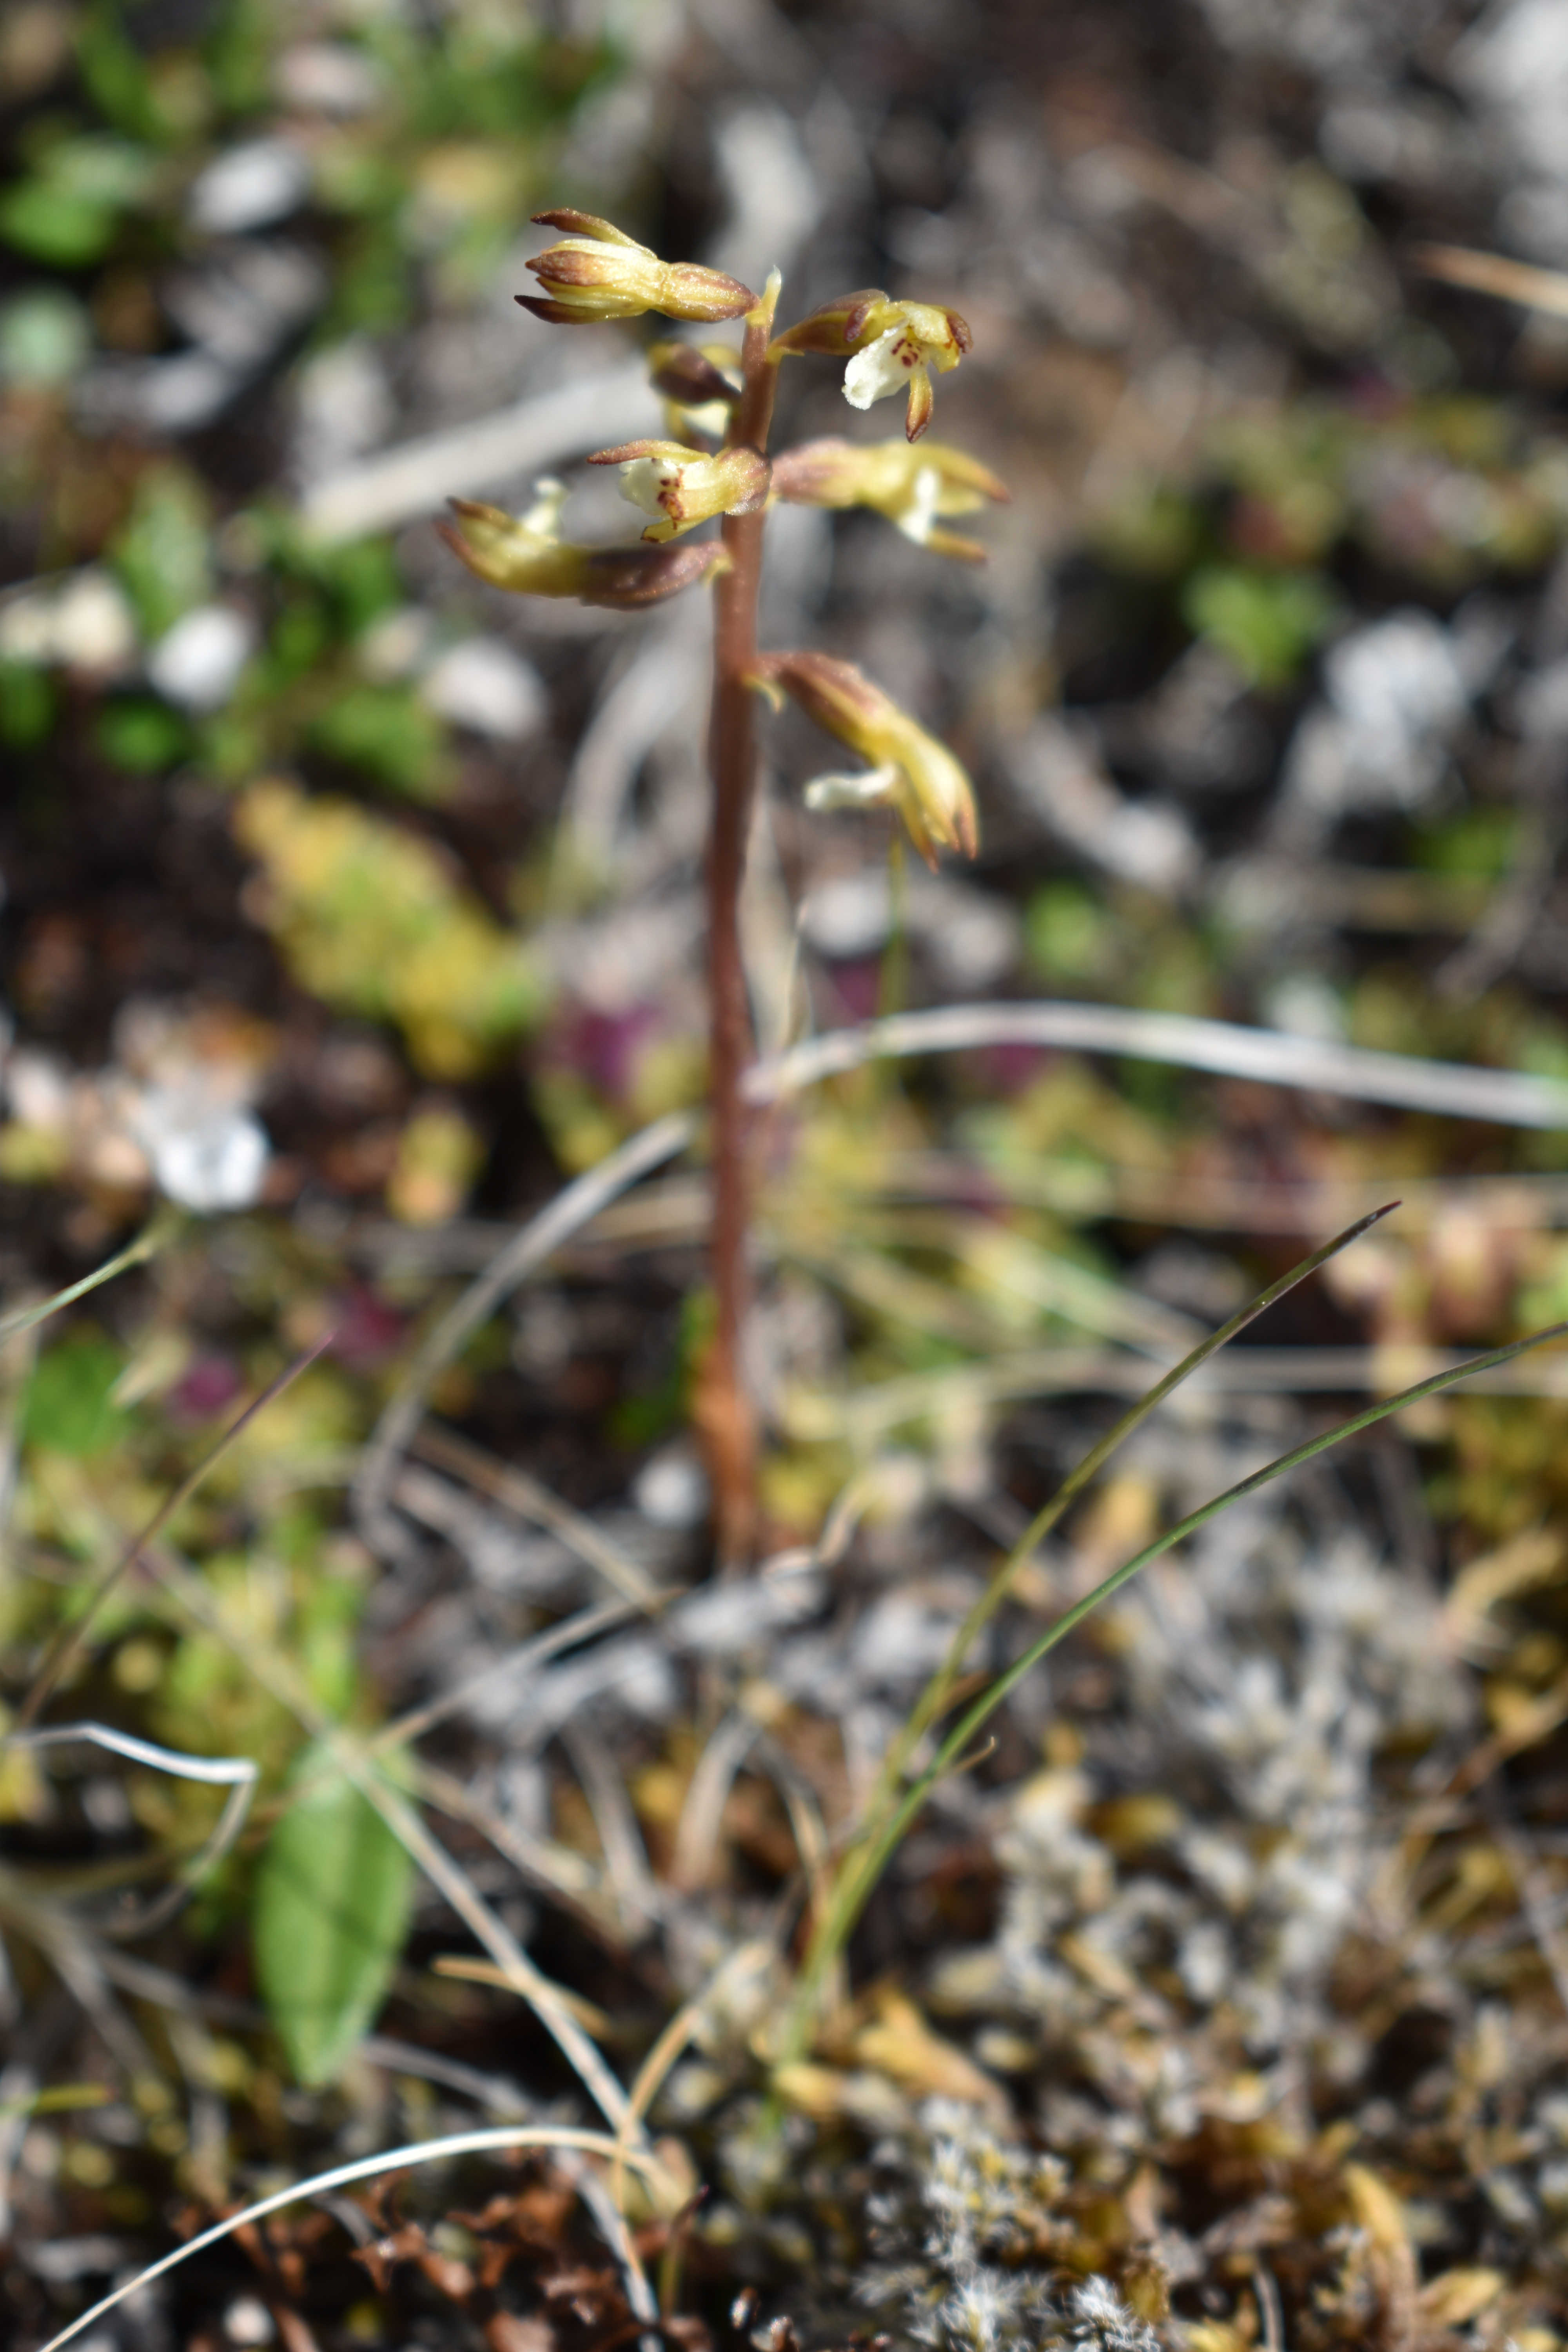
\includegraphics{myndir/blom.JPG}{]} \\
.footer-note-black.white.scriptsize{[} Orkídeutegundin kræklurót, er
fremur sjaldgæf sníkjujurt án blaðgrænu. Kræklurótin finnst nokkuð víða
í héraðinu.{]} {]}{]} \\
??? Orkídeutegundin kræklurót, er fremur sjaldgæf sníkjujurt án
blaðgrænu. \\
\bottomrule
\end{longtable}

class: split-60 with-border middle

.column{[}.content.nopadding{[}{]}{]}

.column{[}.content{[} Áhersla er lögð um allt land á innviðauppbyggingu
og eftirlit með náttúruverndarsvæðum og öðrum stöðum með merkilegt
náttúrufar, svo sem merkum jarðminjum eða ríkulegu fuglalífi. Á
Norðurlandi vestra finnast margir staðir sem tilheyra þessum flokki og
með áframhaldandi uppbyggingu innviða þeirra er hægt að koma í veg fyrir
að landshlutinn dragist aftur úr öðrum. Landverðir á vegum
Umhverfisstofnunar eru ekki starfandi á svæðinu og er það bagalegt. Sem
dæmi má nefna að gerð og viðhald gönguleiða bera þess víða merki, en sú
vinna hefur aðallega fallið í hlut viðkomandi sveitarfélaga. Yfir
háferðamannatímann er eftirliti á Hveravöllum sinnt vikulega af
landverði sunnan úr Kerlingafjöllum. Hveravellir tilheyra þó vissulega
Norðurlandi vestra og eru sennilega annar fjölsóttasti ferðamannastaður
á hálendi Íslands á eftir Landmannalaugum.{]}{]}

\begin{longtable}[]{@{}
  >{\raggedright\arraybackslash}p{(\columnwidth - 0\tabcolsep) * \real{0.06}}@{}}
\toprule
\endhead
class: top background-image: url(myndir/BJ.JPG) background-size:
cover \\
.pull-left{[} .content-box-blue{[} \\
Bjarni Jónsson, forstöðumaður, var kosinn á þing á árinu og lét af
störfum. Við þökkum honum fyrir samstarfið og óskum honum velfarnaðar á
nýjum vettvangi. {]} {]} \\
\bottomrule
\end{longtable}

class: top name: starfsmenn background-image: url(myndir/einar.jpeg)
background-size: contain

.pull-right{[}{]}

\begin{center}\rule{0.5\linewidth}{0.5pt}\end{center}

class: split-40 with-border middle

.column{[}.content{[} \# .black.font-dance{[}Starfsmenn{]} Valtýr
Sigurðsson, líffræðingur, er í hálfu starfi hjá stofunni á móti starfi
sínu hjá BioPol. Hann sinnir rannsóknum á örplasti, botndýrum í sjó,
þara og almennu náttúrufari á svæðinu. {]}{]}

.column{[}.content.nopadding{[}{]}{]}

\begin{center}\rule{0.5\linewidth}{0.5pt}\end{center}

class: split-60 with-border middle

.column{[}.content.nopadding{[}{]}{]}

.column{[}.content{[}{]}{]}

\begin{longtable}[]{@{}
  >{\raggedright\arraybackslash}p{(\columnwidth - 0\tabcolsep) * \real{0.06}}@{}}
\toprule
\endhead
layout: false name: vidfangsefni background-image:
url(myndir/breyttar/kattarauga.JPEG) background-size: cover \\
.white.font-dance.font5{[}Helstu viðfangsefni\ldots{]}
.footer-note-black.white{[} Kattarauga í Vatnsdal er friðlýst
náttúruvætti.{]} \\
\bottomrule
\end{longtable}

layout:false class: split-40 bg-white with-border bottom
background-image: url(myndir/ashildur.JPEG) background-size: cover

.row{[} .font2{[}Farið var af stað með vöktunarverkefni sem að nefnist
\textbf{Vöktun náttúruverndarsvæða} árið 2020. Náttúrustofan hefur tekið
drjúgan þátt í því og safnað gríðarmikið af upplýsingum um nátturfar
þessara svæða ásamt því að gera ástandsmat á stöðunum með tilliti til
margvíslegra ógna meðal annars ágangs ferðamanna.{]}{]}

.row{[} .split-two.with-border{[}{]}{]}

\begin{center}\rule{0.5\linewidth}{0.5pt}\end{center}

class: split-four background-image: url(myndir/Drangey\_sky.JPG)
background-size: contain

.column.bg-main1{[}.content.vmiddle.nopadding{[} .footer-note-R{[}Dróni
var keyptur í tengslum við vöktun náttúruverndarsvæða árið 2020. Hann
hefur verið notaður við kortlagningu og ýmislegt fleira.{]}
.img-fill{[}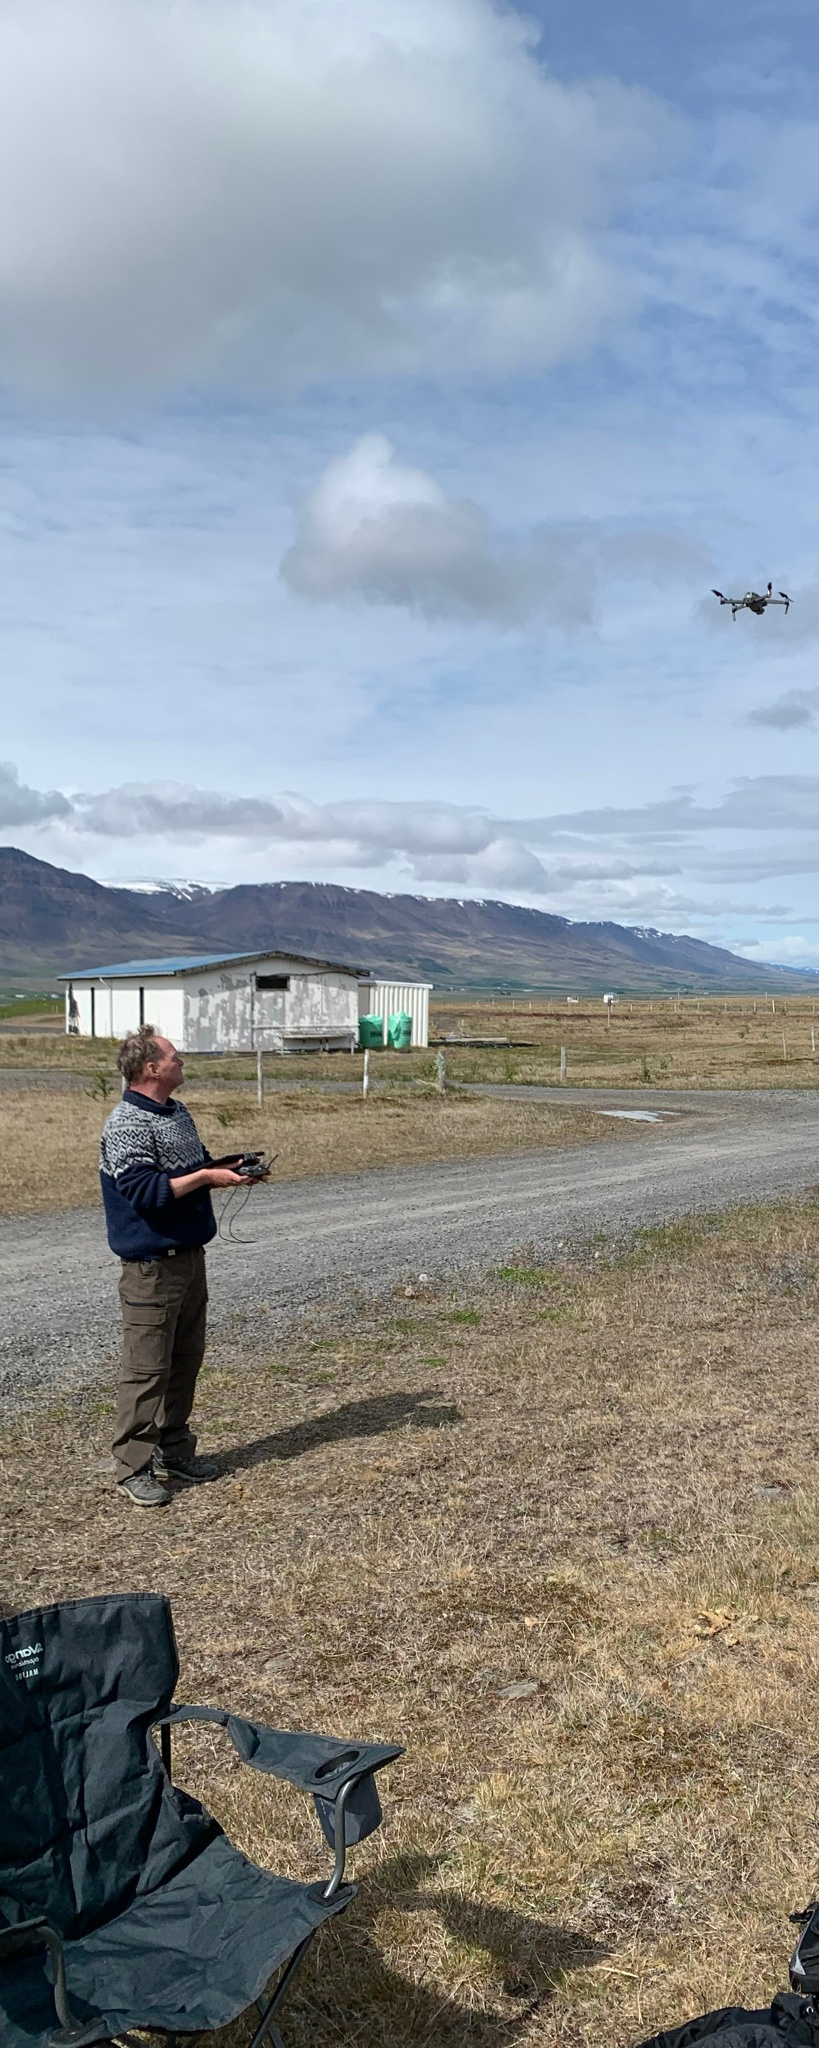
\includegraphics{myndir/droni.JPEG}{]}{]}{]}
.column.bg-main2{[}.content{[}{]}{]}
.column.bg-main3{[}.content.vmiddle.center{[}{]}{]}
.column.bg-main4{[}.content{[} .footnote.Large.white{[}Drangey{]}{]}{]}

\begin{center}\rule{0.5\linewidth}{0.5pt}\end{center}

layout:false class: split-10 background-image: url(myndir/odinshani.JPG)
background-size: cover

.row{[} .content.justify-right.white{[} \#\# Sjaldgæfir gestir og
áhugaverðar athuganir úr fuglalífinu{]}{]} .row.white{[} .split-two{[}
.column{[}{]} .column{[}{]}{]}{]}

\begin{center}\rule{0.5\linewidth}{0.5pt}\end{center}

class: split-three white

.column{[}.nopadding{[}
.img{[}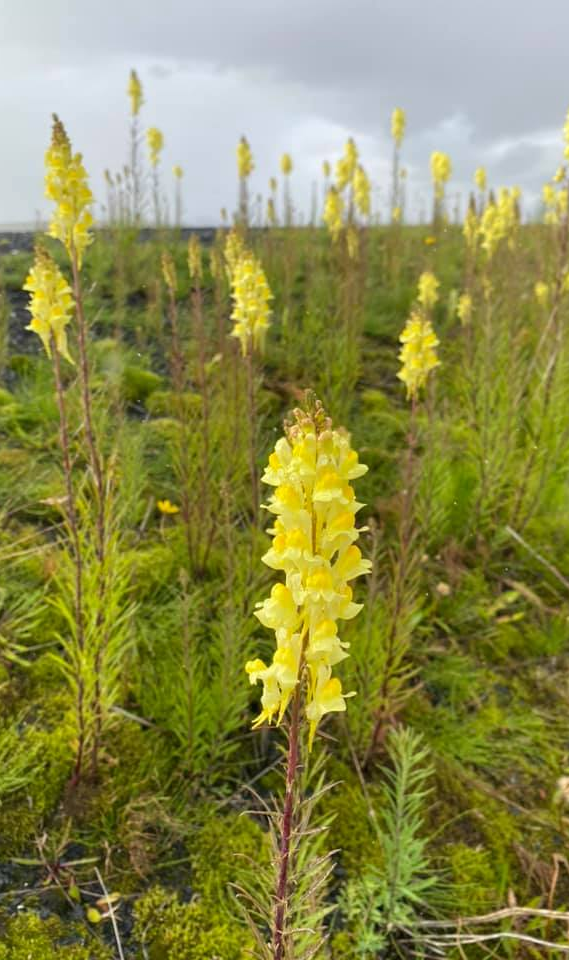
\includegraphics{myndir/breyttar/gullspora.png}{]}
.footer-note{[}Gullsporablóm{]}{]}{]}
.column.bg-blue{[}.content.vmiddle{[}.Large{[}.yellow{[}Sjaldgæfar
plöntur og slæðingar {]}voru víða skráðar samhliða öðrum rannsóknum,
merkilegast má telja fágætar jurtir sem eru að berast víða inn um
hálendið með erlendum ferðamönnum. Má hér helst geta
\textbf{fagurfífils}, \textbf{regfangs} afbrigðis og \textbf{sólfylgju}
sem nú eru á Hveravöllum. Áhugaverðasta plantan sem fannst á láglendi
var \textbf{stúfa} en stúfan hefur annars einungis vaxtarstaði á
Suðurlandi. Gullsporablóm hefur nýlega fundist á tveimur stöðum á
Norðurlandi vestra. Áður var það aðeins fundið á tveimur stöðum á
landinu.{]} .img{[}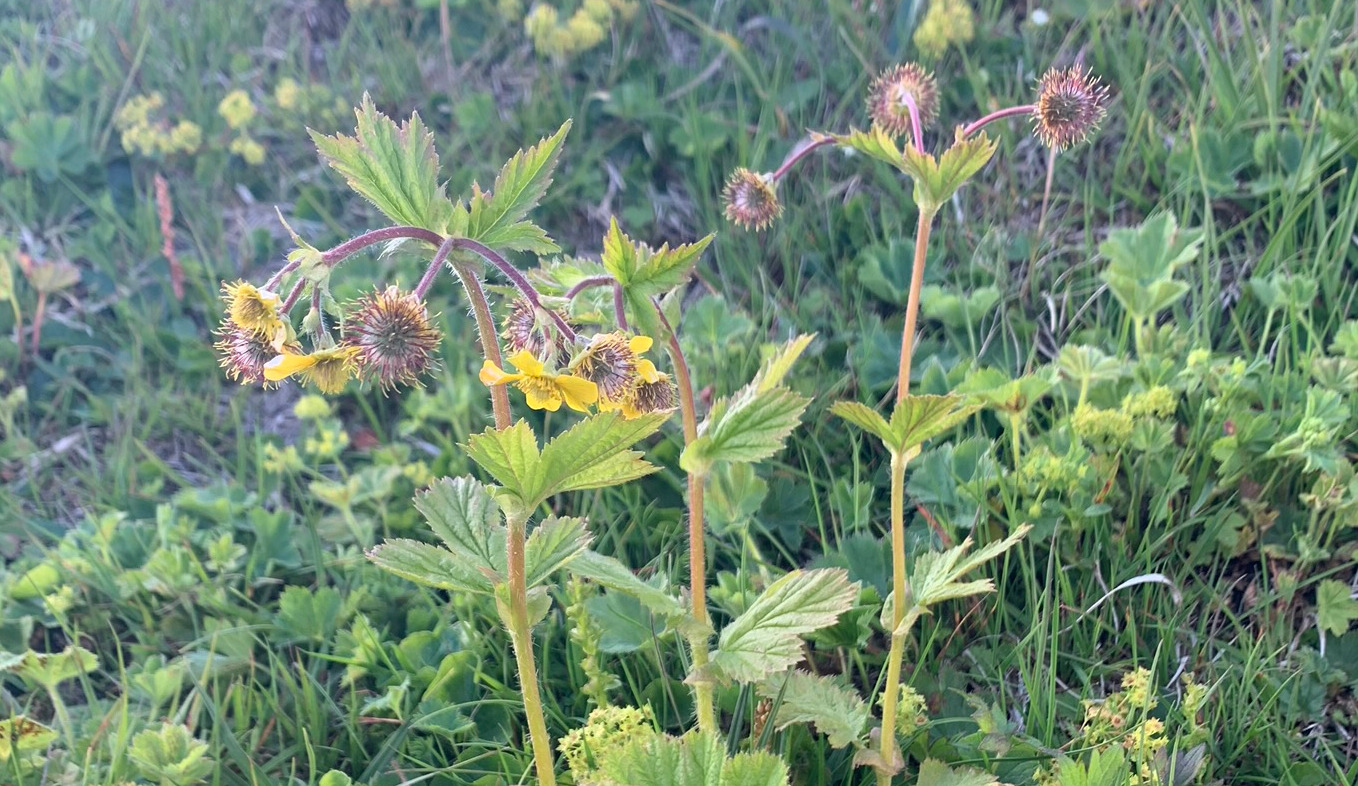
\includegraphics{myndir/solfyglja.JPEG}{]}
Sólfylgja{]}{]} .column.bg-green{[}.content{[}
.img{[}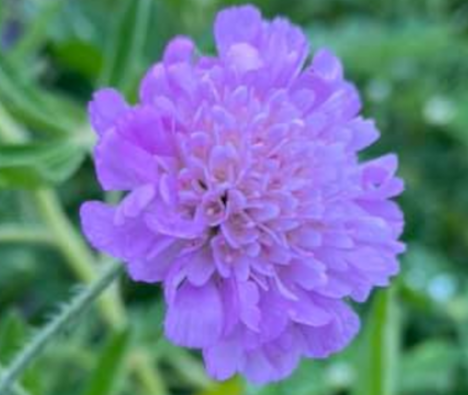
\includegraphics{myndir/stufa.png}{]}\\
Stúfa .img{[}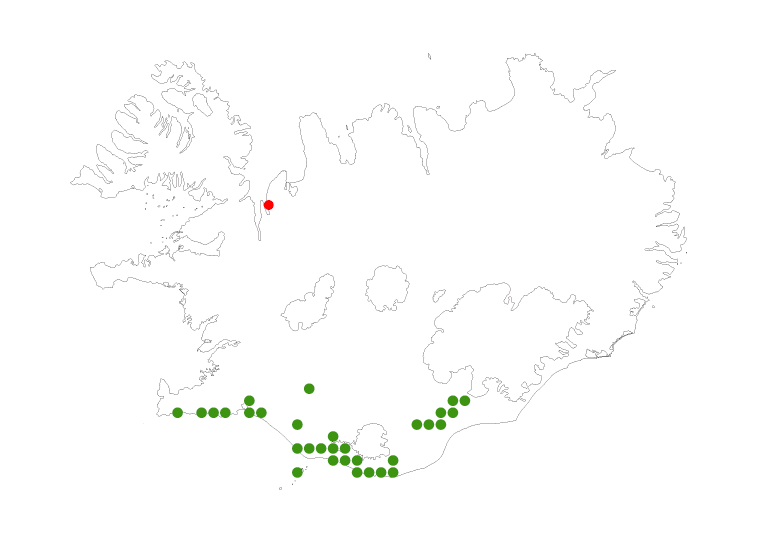
\includegraphics{myndir/kort.png}{]}\\
Útbreiðsla stúfu{]}{]}

\begin{longtable}[]{@{}
  >{\raggedright\arraybackslash}p{(\columnwidth - 0\tabcolsep) * \real{0.06}}@{}}
\toprule
\endhead
layout:false class: split-60 bg-white with-thick-border
background-image: url(myndir/ashildur.JPEG) background-size: cover \\
.row{[} .split-three.with-thick-border{[} .column{[}.nopadding{[} \\
.img-fill{[}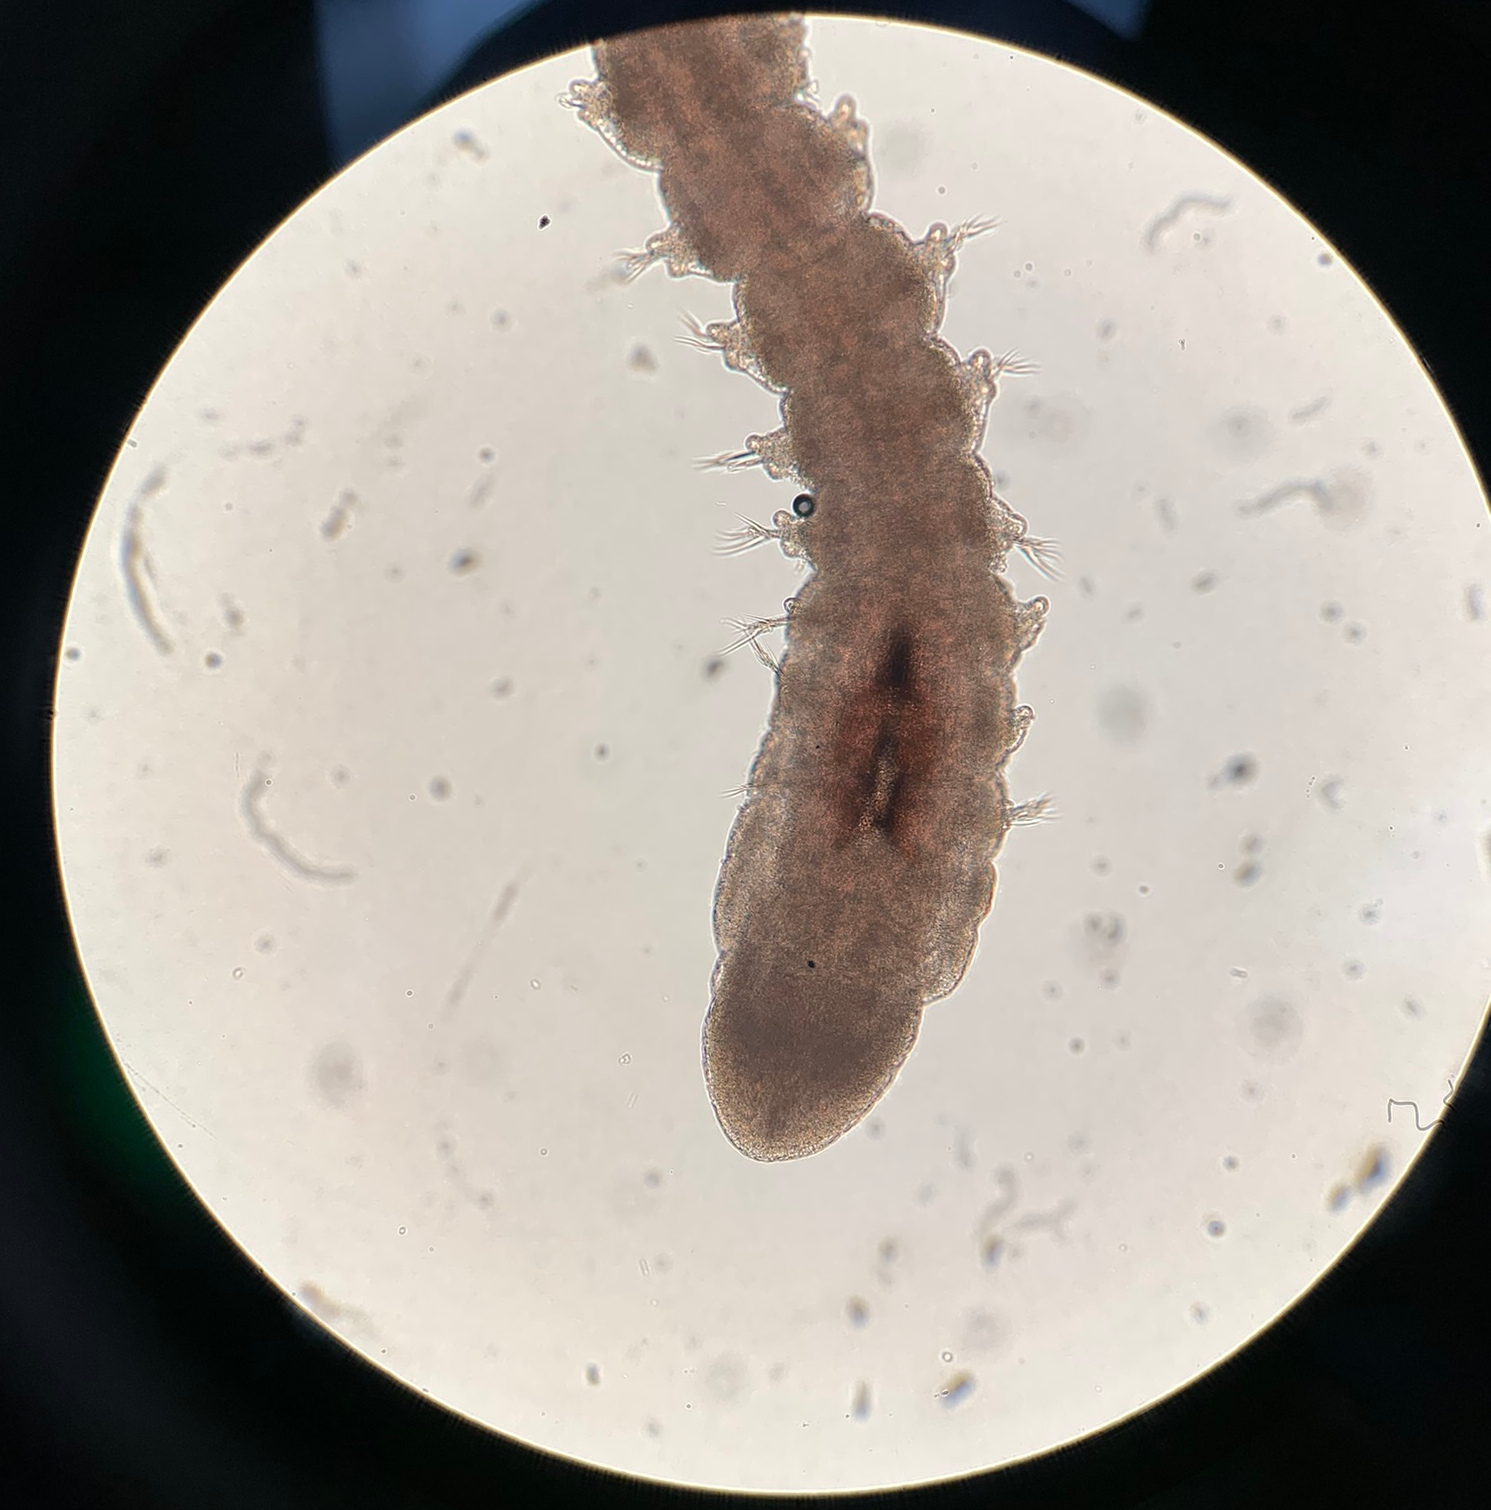
\includegraphics{myndir/burstaormur.jpeg}{]}
.footer-note-black.white.scriptsize{[}Burstaormur úr
Kolgrafafirði.{]} \\
{]}{]} \\
.column.bg-white{[}.nopadding{[} \\
.img-fill{[}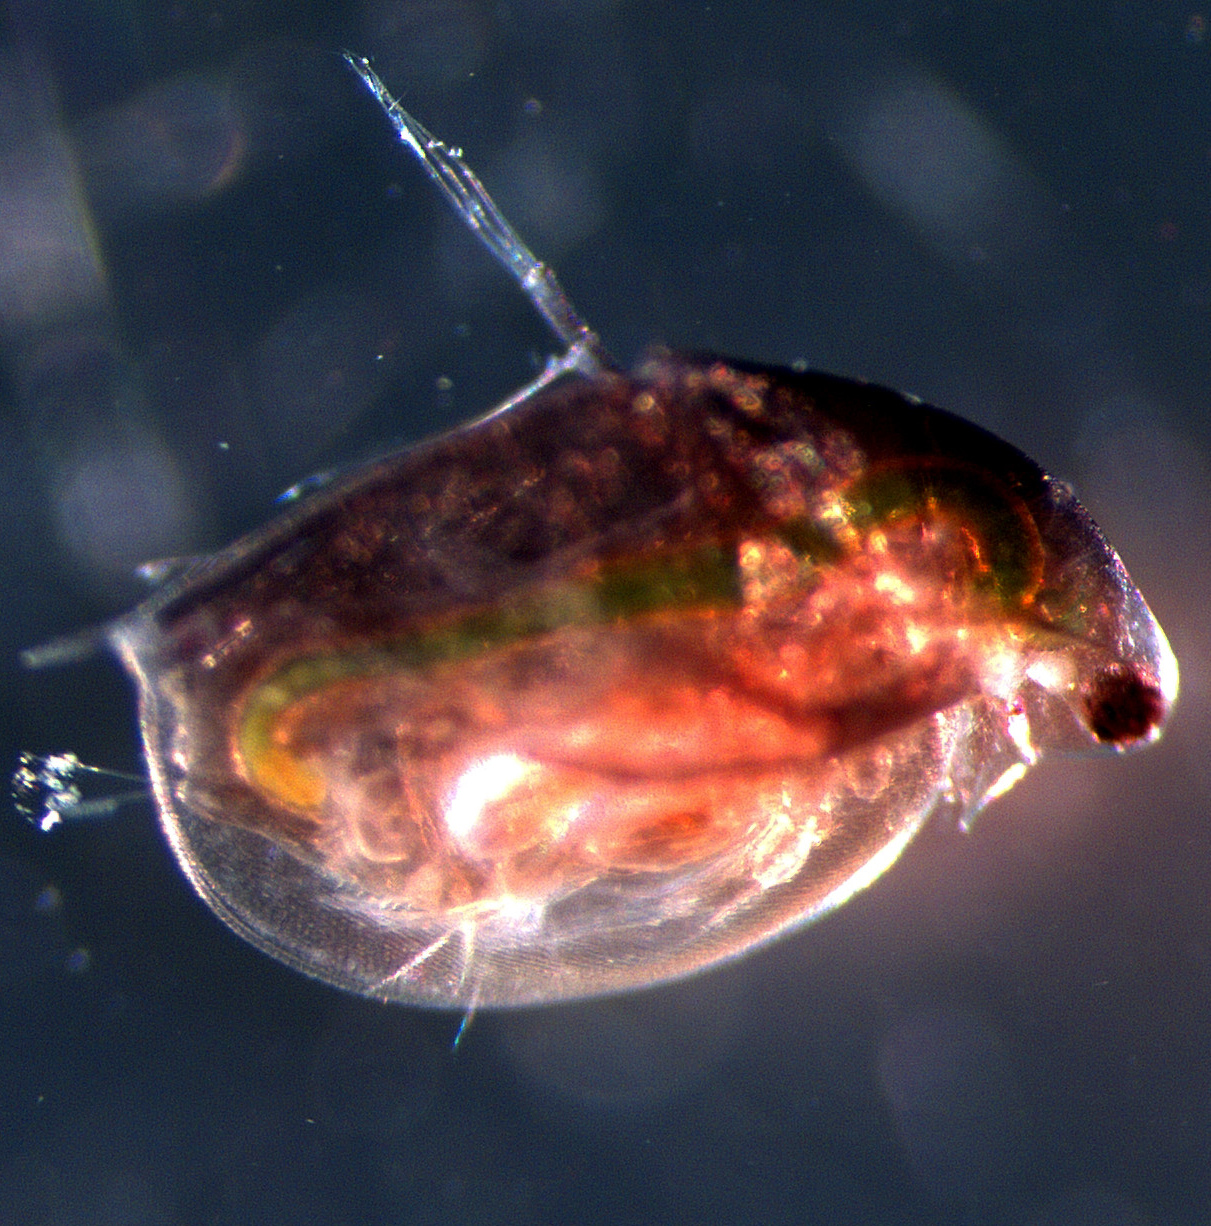
\includegraphics{myndir/DAPHNIA_PULEX.JPG}{]}
.footer-note-black.white.scriptsize{[}Stutthalafló úr Reiðarvatni á
Hofsafrétti.{]} {]} \\
{]} .column.bg-white{[}.nopadding{[} \\
.img-fill{[}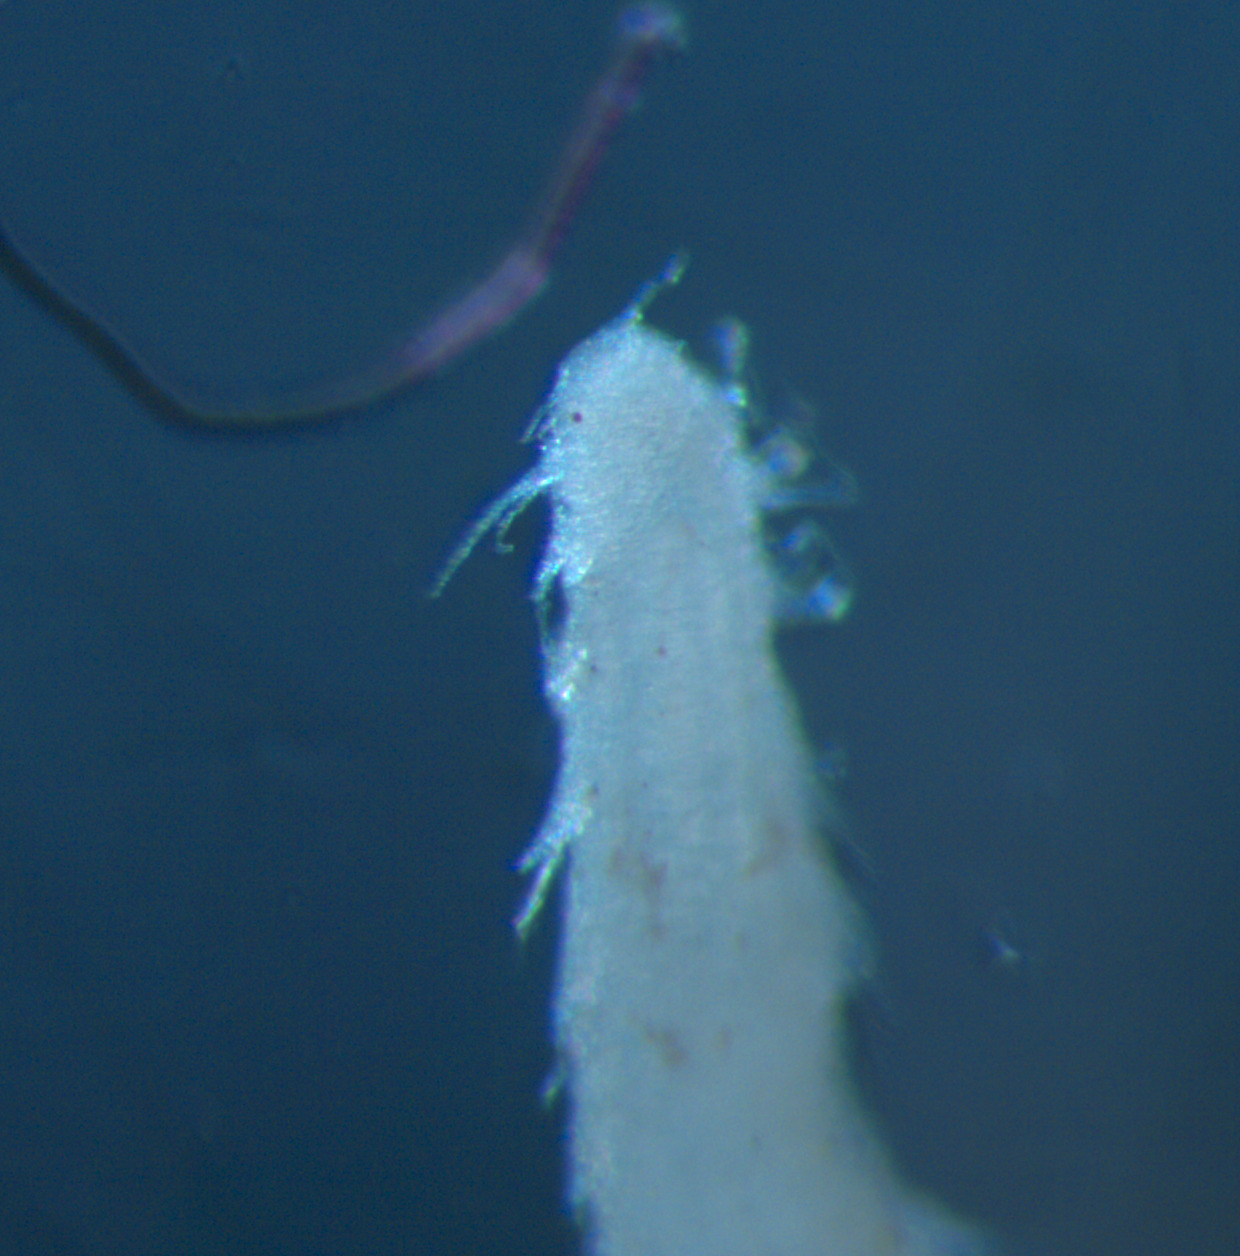
\includegraphics{myndir/Clongocirrata.jpg}{]}
.footer-note-black.white.scriptsize{[}Microphthalmus sp.{]} {]}{]}
{]}{]} \\
.row{[} \\
.yellow.font2{[}Náttúrustofan tekur þátt í greiningum á botndýrum í sjó
í verkefni tengdu Náttúrustofu Vesturlands og Háskólasetrinu í
Stykkishólmi. Einnig er lítillega fengist við greiningar á smádýrum úr
vötnum{]} \\
{]} \\
\bottomrule
\end{longtable}

layout:false background-image: url(myndir/reykjafoss.jpeg)
background-size: contain

.split-three{[} .column.bg-white{[}.content.pad1{[}{]}{]}{]}{]}

\begin{center}\rule{0.5\linewidth}{0.5pt}\end{center}

class: split-three, middle name: erindi background-image:
url(myndir/breyttar/bolugil.JPG) background-size: cover

.column.bg-white{[} .large{[}.content.pad1{[}{]}{]}{]} .column{[}{]}
.column{[}{]}

\begin{longtable}[]{@{}
  >{\raggedright\arraybackslash}p{(\columnwidth - 0\tabcolsep) * \real{0.06}}@{}}
\toprule
\begin{minipage}[b]{\linewidth}\raggedright
class: split-three, middle name: fjolm background-image:
url(myndir/breyttar/eyrarros.JPEG) background-size: cover .column{[}
.footer-note-black.white.scriptsize{[} Eyrarrós á Hofsafrétti.{]}{]}
.column{[}{]}
\end{minipage} \\
\midrule
\endhead
name: ymislegt layout:false class: split-40 bg-white with-thick-border
bottom background-size: cover \\
.row{[} \\
.column.pad1{[}\# Ýmislegt fleira .large{[} \\
Náttúrustofan tók þátt í \textbf{arnarmerkingum} með starfsmönnum
Náttúrufræðistofnunar Íslands. Alls voru merktir arnarungar á 4 hreiðrum
á okkar svæði. Ernir sáust víða og má teljast merkilegt hvað þeir eru
tíðir á Arnarvatnsheiði og á Miðhálendinu til dæmis við Ásbjarnarvötn í
um 700 metra hæð yfir sjávarmáli. \\
Fullorðinn fálkakarl fannst slasaður í Hrútafirði. Hann var fóðraður og
hjúkrað í nokkrar vikur og komið til heilsu. Hann var svo fluttur í
Húsdýragarðinn. \\
{]} {]} {]} \\
.row{[} .split-three.with-thick-border{[} .column{[}.nopadding{[} \\
.img-fill{[}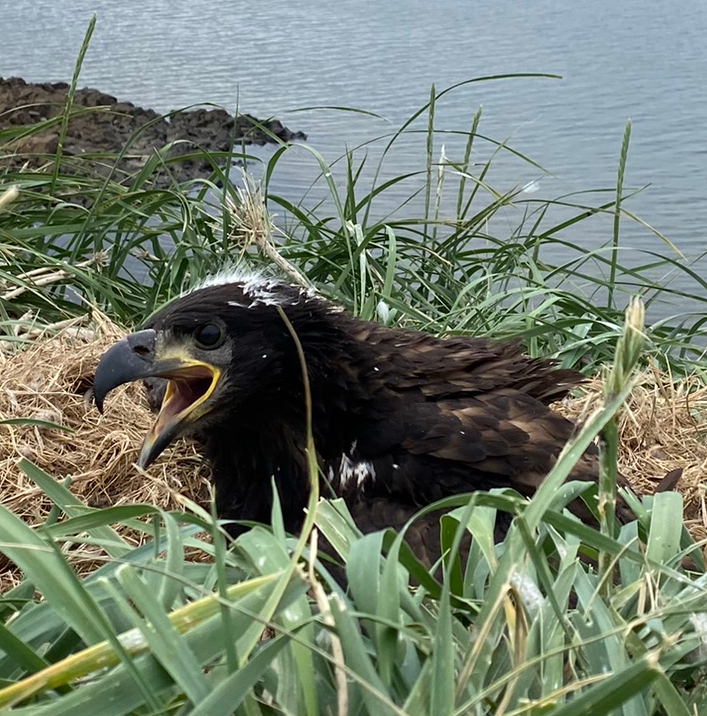
\includegraphics{myndir/breyttar/arnarungi.JPEG}{]}
.footer-note-black-R.white.scriptsize{[} Merktur arnarungi í
hreiðri.{]} \\
{]}{]} \\
.column.bg-white{[}.nopadding{[} \\
.img-fill{[}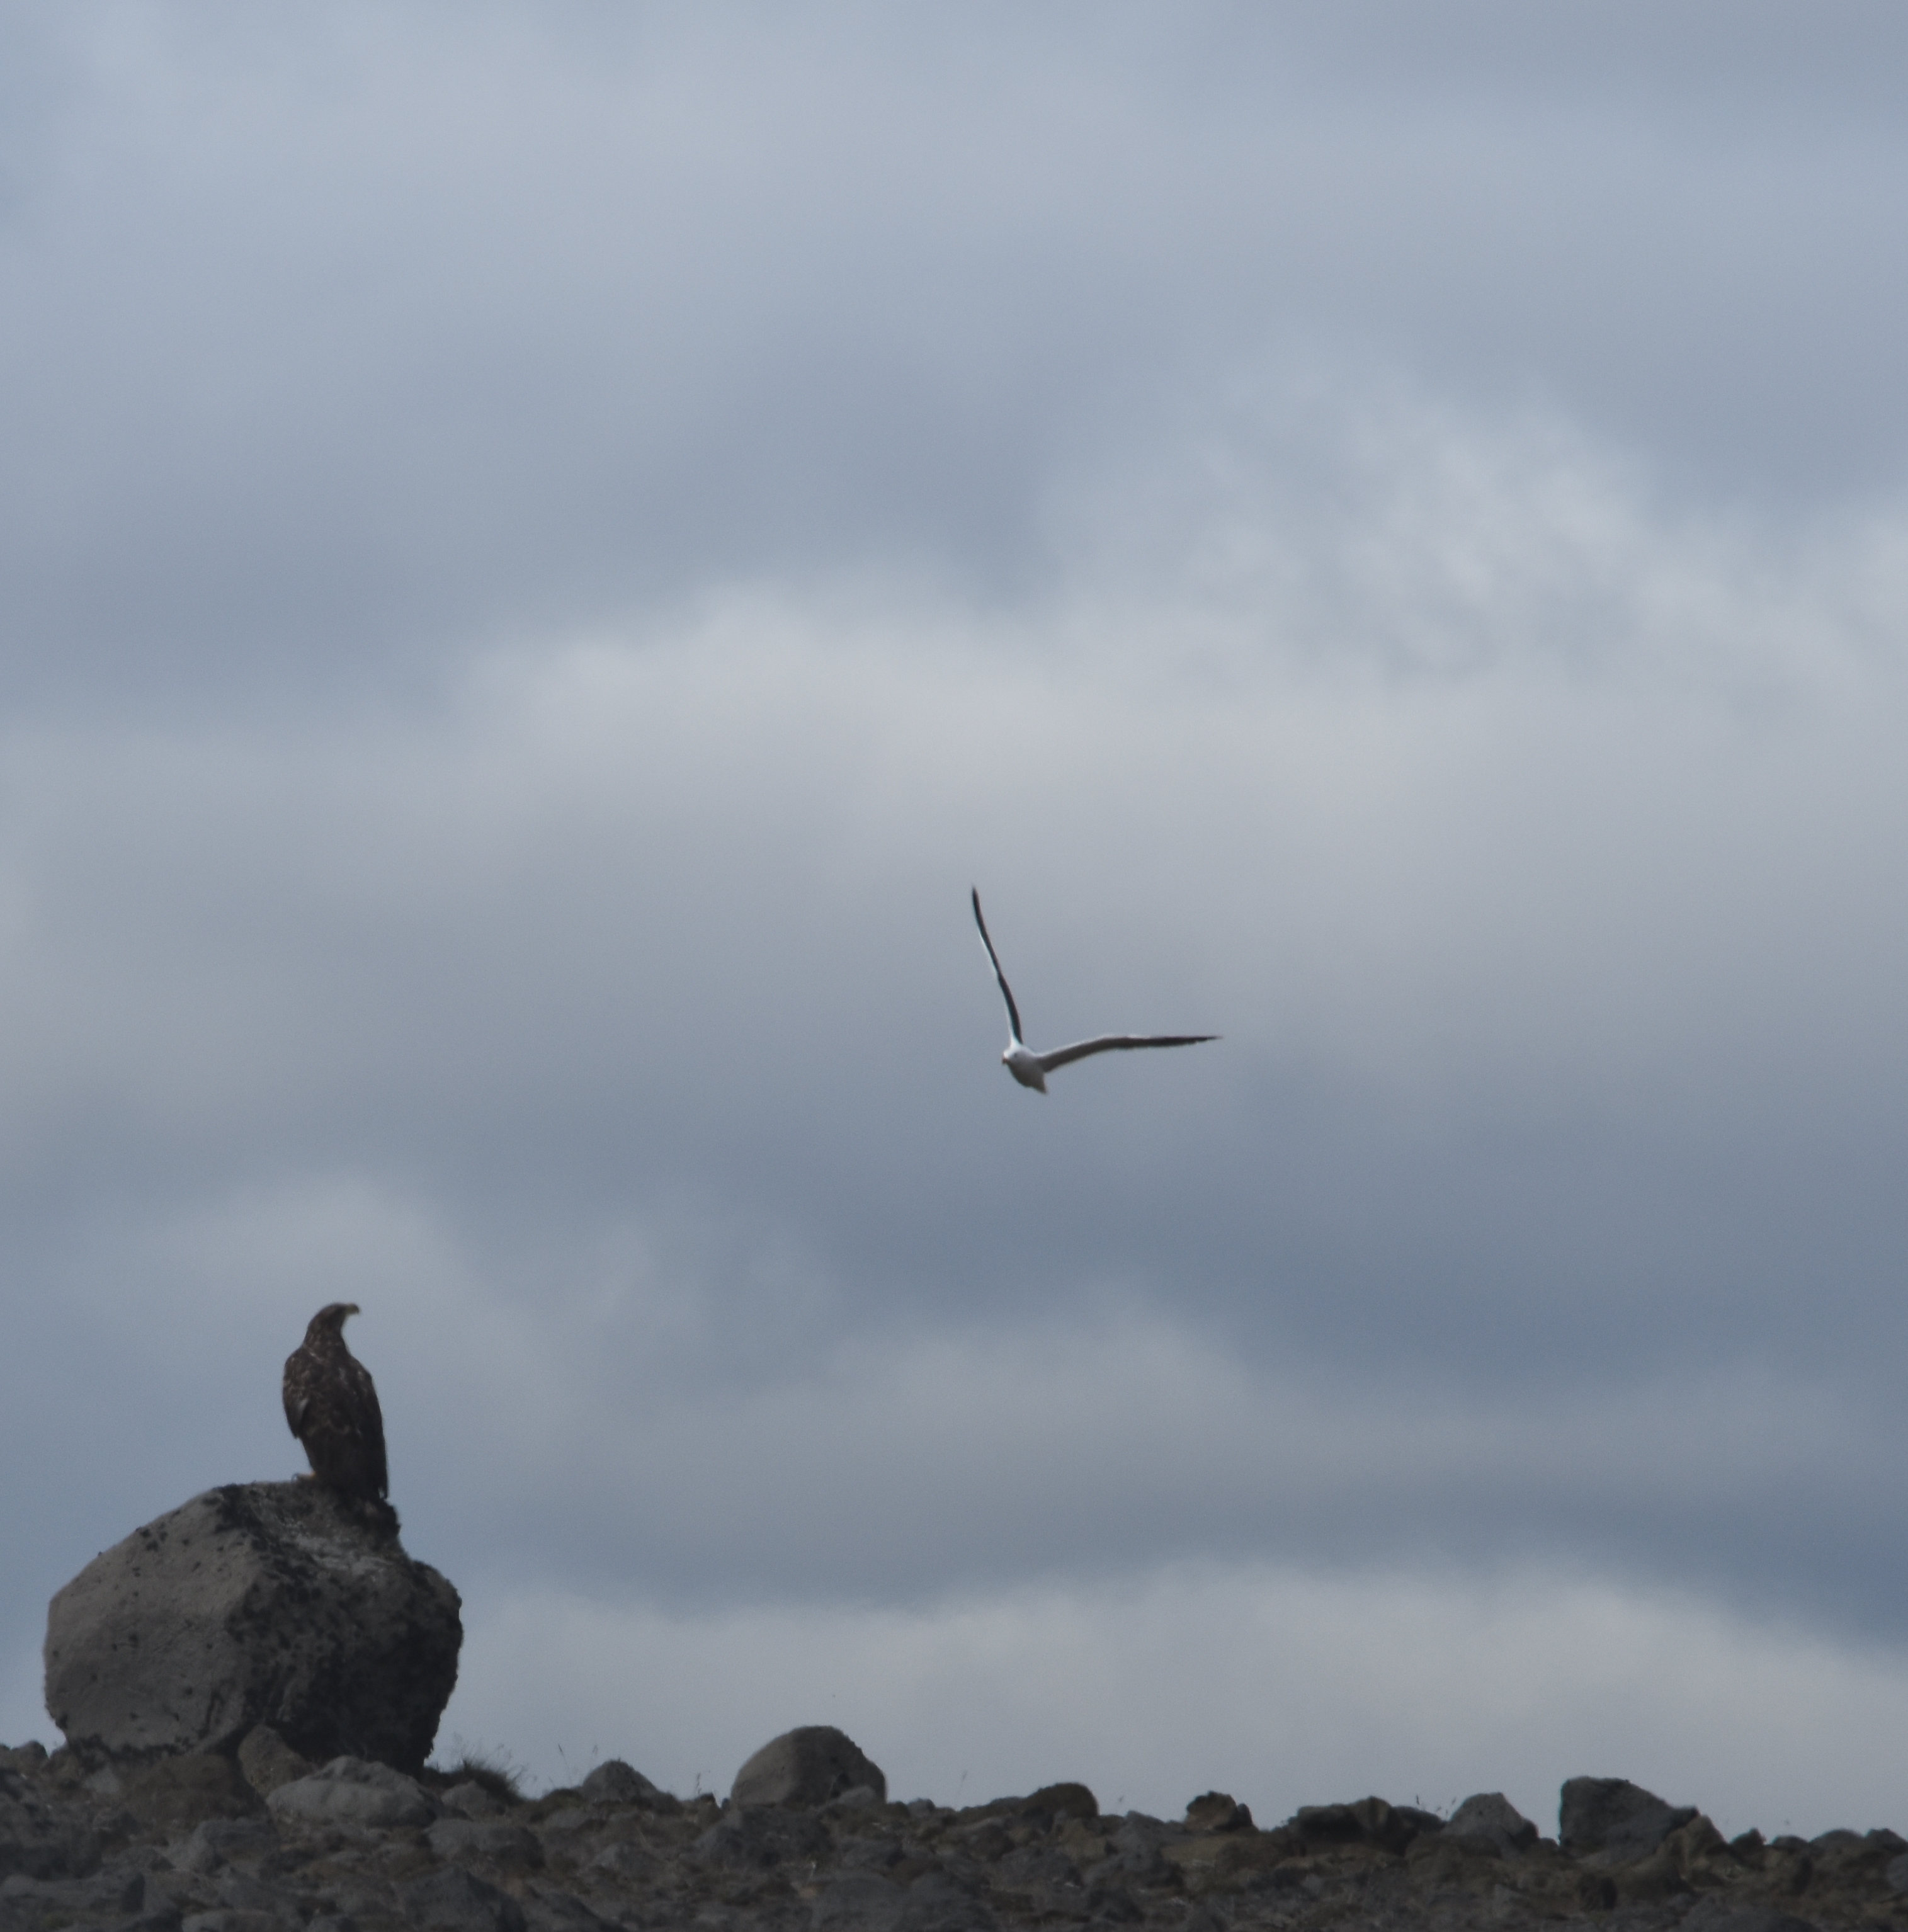
\includegraphics{myndir/haforn.JPG}{]}
.footer-note-black-R.white.scriptsize{[} Haförn verður fyrir árás frá
svartbaki á miðhálendinu.{]} {]} \\
{]} .column.bg-white{[}.nopadding{[} \\
.img-fill{[}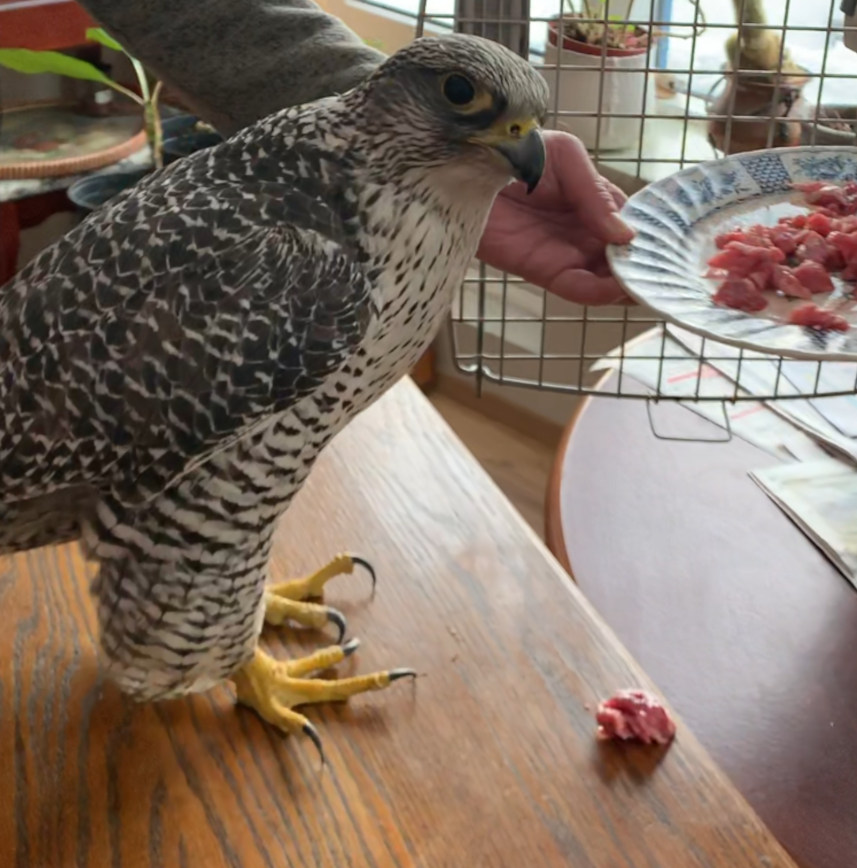
\includegraphics{myndir/falki.PNG}{]} \\
{]}{]} {]}{]} \\
\bottomrule
\end{longtable}

layout:false class: split-60 bg-white with-thick-border, middle

.row{[} .split-three.with-thick-border{[} .column{[}.nopadding{[}
.footer-note-black-R.white.scriptsize{[}Blaðfar, birki. Bakkabrúnir í
Víðidal.{]}
.img-fill{[}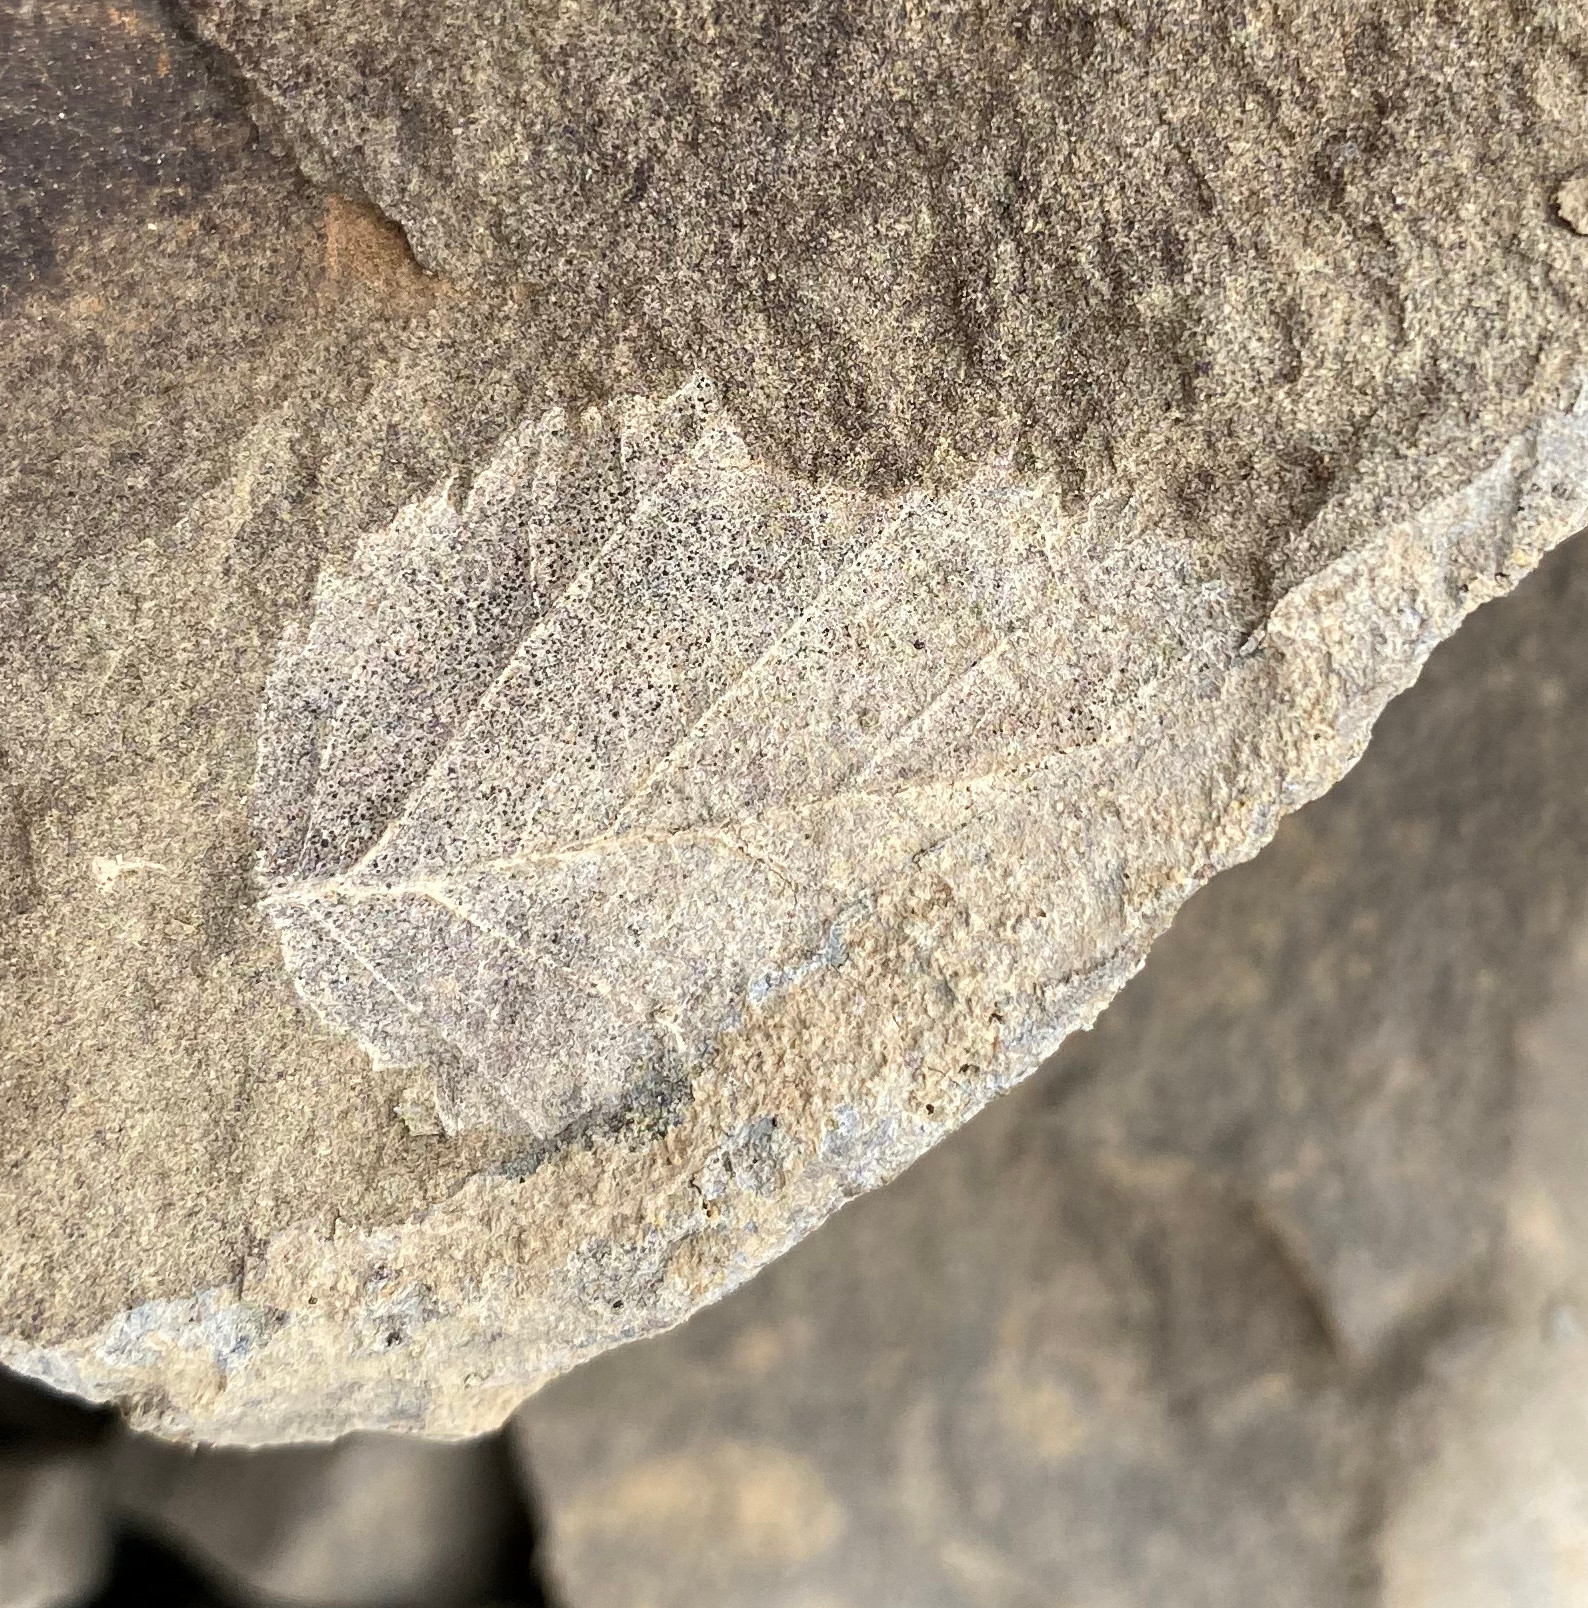
\includegraphics{myndir/breyttar/bakkabrunir.jpg}{]}{]}{]}{]}{]}

.row{[} .split-two.border-white{[} .column{[} .large{[}{]}{]}{]}{]}

\begin{center}\rule{0.5\linewidth}{0.5pt}\end{center}

layout:false class: split-40 bg-white with-thick-border background-size:
cover

.row{[}.large.vmiddle{[} .Large{[}Mjög fallegt stuðlaberg{]} finnst á
nokkrum stöðum. Þekktustu staðirnir eru Hofsós, Kálfshamarsvík og
Borgarvirki. Færri vita af geisifallegu stuðlabergi í \textbf{Nesbjörgum
í Vesturhópi} eða \textbf{Káraborg á Vatnsnesi}, eins má nefna merkilegt
stuðlaberg í stórri námu hjá \textbf{Friðmundarvötnum á Auðkúluheiði}
við leiðina um Kjalveg. Eða merkilegt stuðlaberg sem að
\textbf{hafnargarðurinn á Skagaströnd} er byggður utan í.{]}{]}

.row{[} .split-three.with-thick-border{[}{]}{]}

\begin{center}\rule{0.5\linewidth}{0.5pt}\end{center}

layout:false class: split-60 bg-white with-thick-border, middle

.row{[} .split-three.with-thick-border{[} .column{[}.nopadding{[}
.footer-note-black-R.white.scriptsize{[}Kóngasvarmi á Hvammstanga.{]}
.img-fill{[}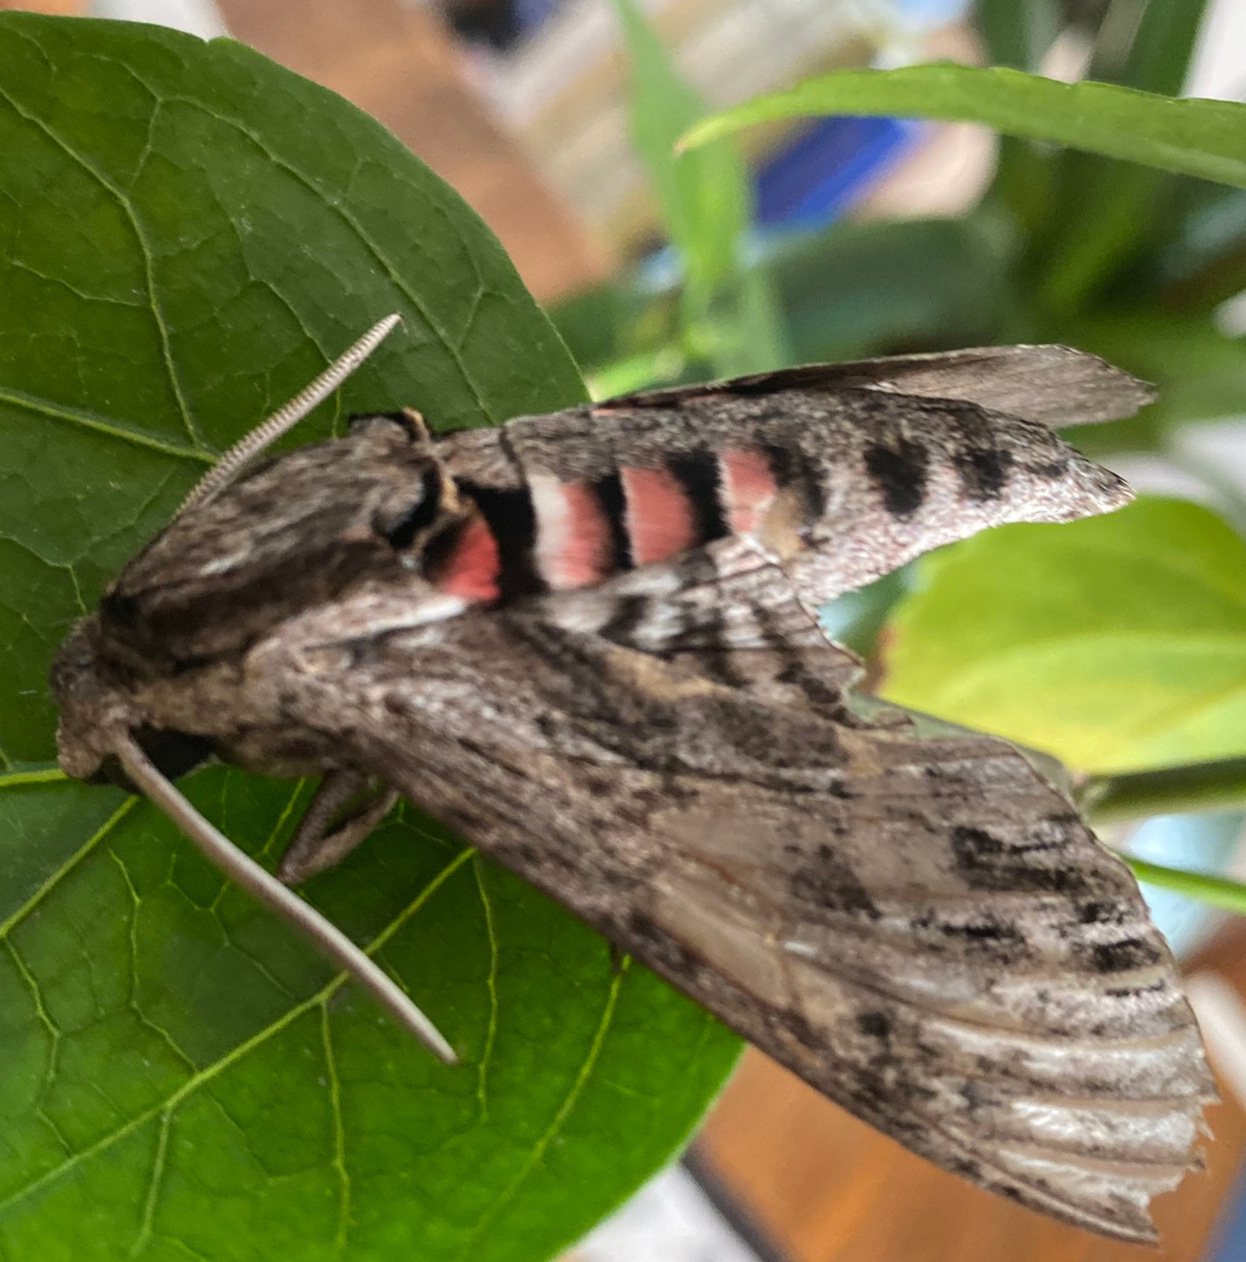
\includegraphics{myndir/kongasvarmi.jpeg}{]}{]}{]}{]}{]}

.row{[} .split-two.border-white{[} .column{[} .large{[} Þessi sjaldgæfi
\textbf{kóngasvarmi} fannst á Hvammstanga. Hann er með allra stærstu
næturfiðrildum sem hér finnast, með 8 til 10 cm vænghaf og er eitt
stærsta skordýr Evrópu. Þetta er sjaldgæfur flækingur sem berst með
hlýum vindum síðsumars. Náttúrustofan tekur við ábendingum með glöðu
geði og hjálpar til við greiningar á dýrum stórum sem smáum.{]}{]}{]}{]}

\begin{longtable}[]{@{}
  >{\raggedright\arraybackslash}p{(\columnwidth - 0\tabcolsep) * \real{0.06}}@{}}
\toprule
\endhead
layout: false class: split-two with-thick-border middle \\
.row{[} .split-two{[} .column.bg-white{[} \\
\# Lífríki og loftslagsbreytingar NNV hefur í sífelldri athugun áhrif
loftslagsbreytinga á útbreiðslu dýra og plantna. Viðbúið er að
hánorrænar fuglategundir og fjallaplöntur hörfi til kaldari svæða á
komandi árum. Í því sambandi má nefna sólskríkju/snjótittling og
fjallaplönturnar jöklasóley og fjallavorblóm. Náttúrustofan hefur sinnt
athugunum á sífrera í gróðurvinjum hálendisins en sífrerinn er
mikilvægur fyrir gróður og fuglalíf á miðhálendinu. \\
{]} \\
.column{[}.nopadding{[} \\
.img-fill{[}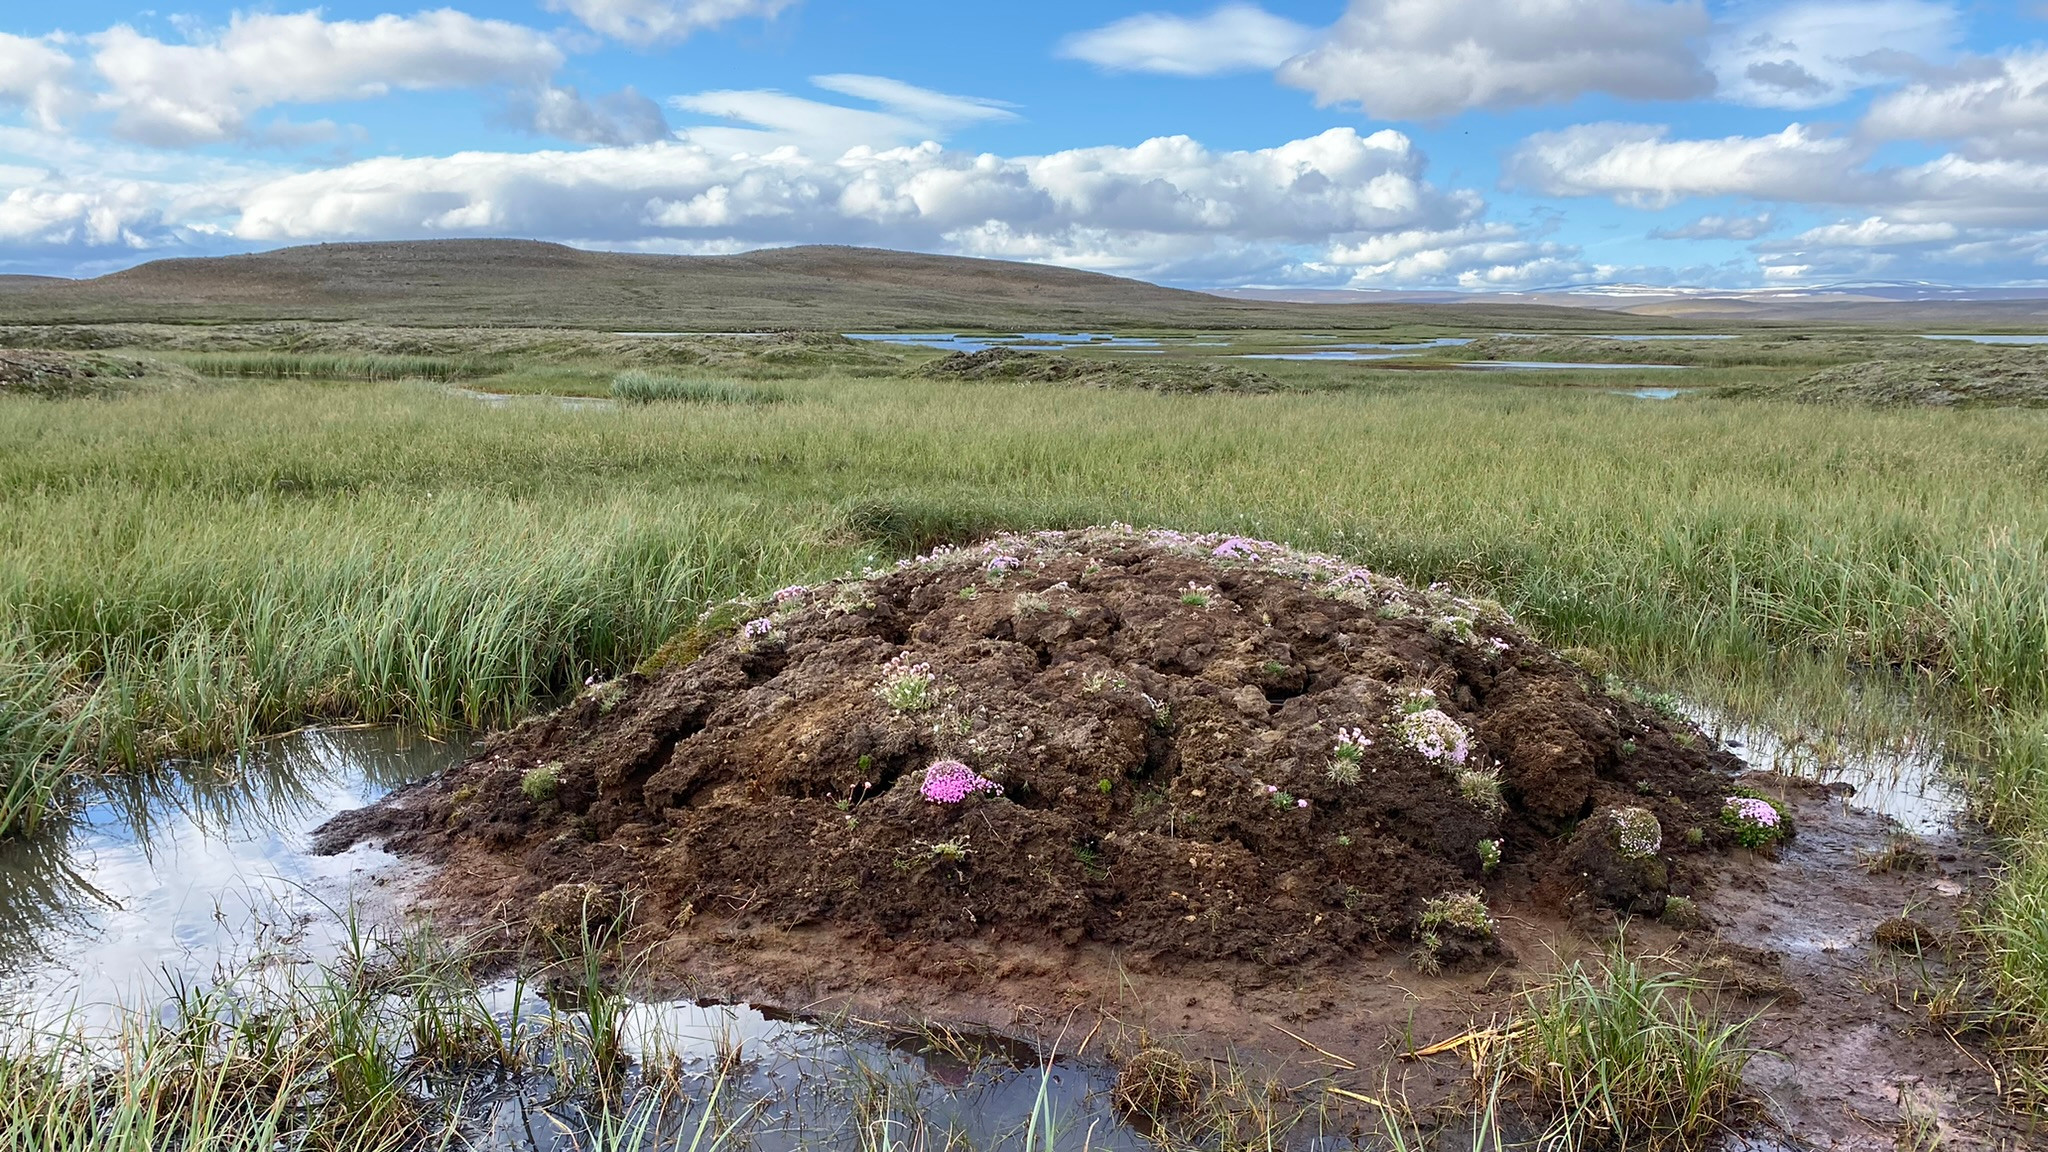
\includegraphics{myndir/breyttar/rust.JPEG}{]} \\
.footer-note-black.white.scriptsize{[}Nýmynduð rúst í
Orravatnsrústum.{]} \\
{]} {]} \\
{]} {]} \\
.row{[} .split-two{[} \\
.column{[}.nopadding{[} \\
.img-fill{[}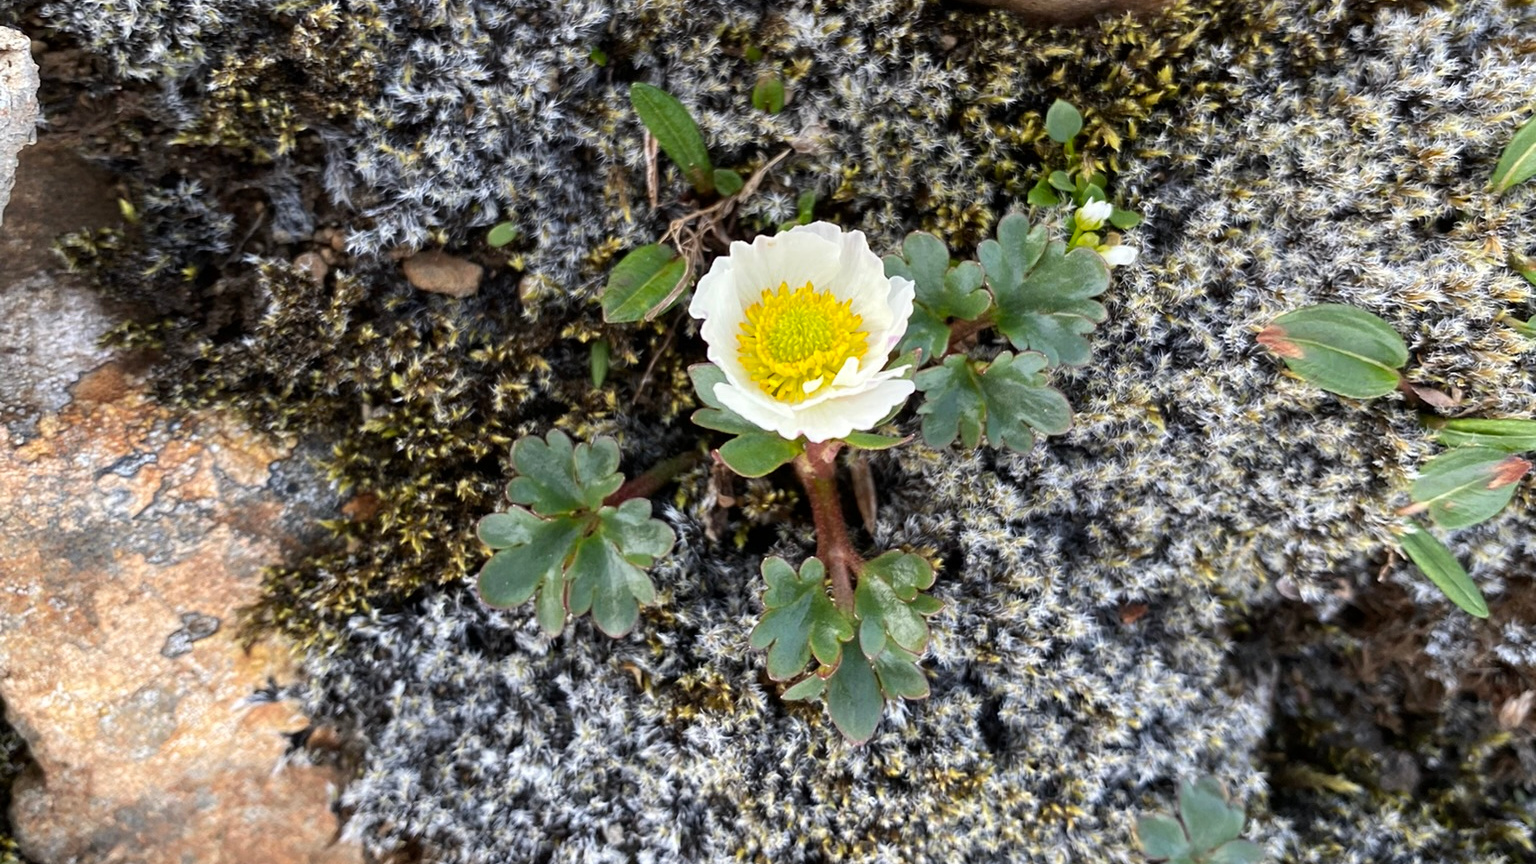
\includegraphics{myndir/breyttar/joklasoley.JPEG}{]} \\
.footer-note-black.white.scriptsize{[}Jöklasóley í 900 metra hæð yfir
sjávarmáli.{]} \\
{]} {]} \\
.column{[}.nopadding{[} \\
.img-fill{[}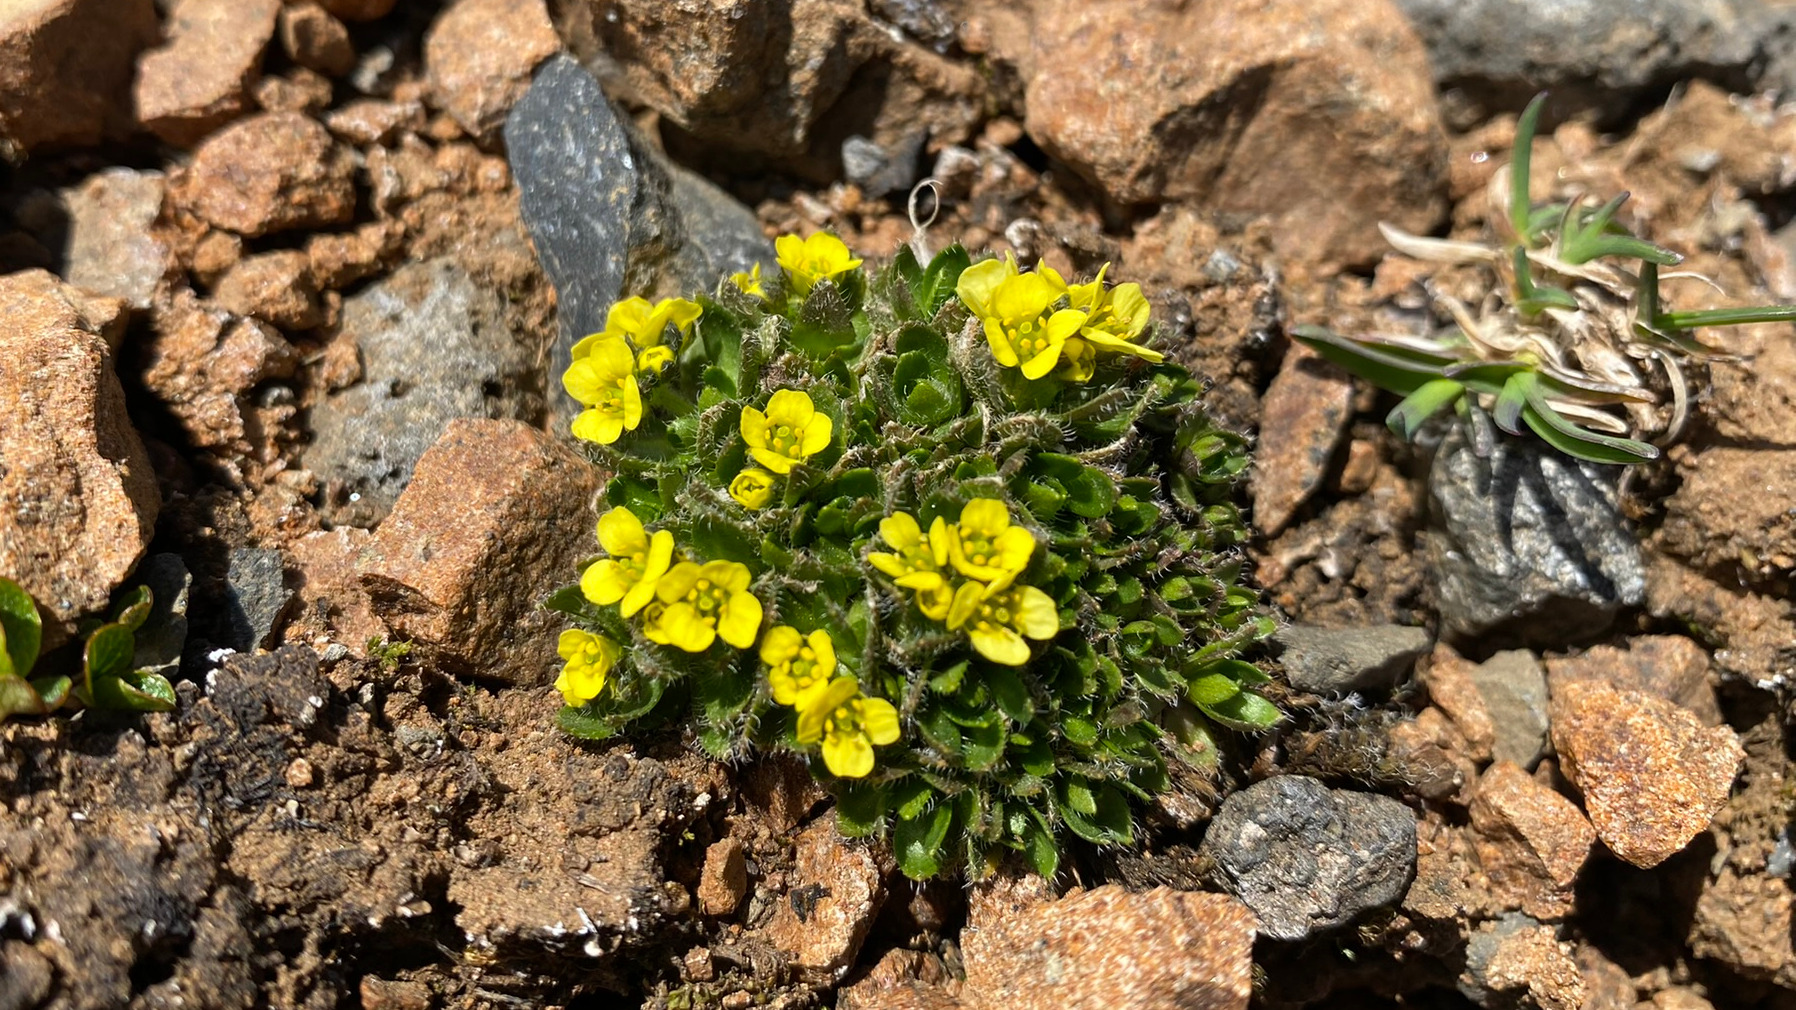
\includegraphics{myndir/breyttar/fjallavorblom.JPEG}{]} \\
.footer-note-black.white.scriptsize{[}Fjallavorblóm.{]} \\
{]} {]} \\
{]} {]} \\
\bottomrule
\end{longtable}

layout:false class: split-50 bg-white background-image:
url(myndir/ashildur.JPEG) background-size: cover

.row{[}{]}

.row{[} .split-three{[} .column{[}{]}{]}{]}

\end{document}
